\section{Components}
\begin{figure}

\includegraphics[scale=0.17]{Overview} 
\caption{system overview}
\end{figure}

%-----

\subsection{Chip-Card}
We use simple memory cards with $I^2$C-Bus and form factor ID-1 as specifyed in \cite{ISO7816-1}\cite{ISO7816-2}. They are quite cheap (less then 1\euro{} per Card) and are not secure. Their contents might be easily read or modifyed. So everyone can read and check what we write on their card.

The card contains a so called \textit{AuthBlock} embedded in a ASN.1-BER\cite{ASN.1BER} octals-string object
The \textit{AuthBlock} has the following structure:\\
\begin{tabular}{|l|c|l|} \hline
name & size & description \\ \hline 
UID            & 2 bytes & index to the \textit{TicketDB} \\
ticket         & 32 bytes & ticket containing encrypted timestamp \\
$r_{key}$ & 32 bytes & random key for $r_{ID}$ decryption \\
$r_{ID}$   & 32 bytes & encrypted user pseudonym \\
HMAC        & 32 bytes & $HMAC_{AuthBlockKey}(UID \parallel ticket \parallel r_{key} \parallel r_{ID})$\\ \hline
\end{tabular} 

%-----

\subsection{realtimeclock (RTC)}
The realtimeclock is implemented in software by using one of the microcontrollers timers. A timer interrupt function increments a 64bit value every millisecond (this counter will wrap arround in about 584.542.046 years, which should be quite enough for us). Additionaly the counters value is periodically\footnote{the value is backed up every $3FFFFF_{(16)}$ milliseconds wich is about every 1.165 hours} written to the microcontrollers EEPROM and read back after reset. On reset we also add the value $3FFFFF_{(16)}$ to the counter to avoid having more then one time the same timestamp.

The backup storage is implemented in a ringbuffer structure with an additional index byte. 
The index byte indicates which cell of the ringbuffer is to use. After writing a value to a cell it is read back and checked. If the check fails the index byte is incremented by one and the next cell is used. The EEPROM is specified to be written 100,000 times so one cell may work for 116,508.4 hours which is about 13.29 years. So with a ringbuffer of 20 cells we should be able to operate for about 265.82 years which should be sufficient for most applications (if not the ringbuffer could be easily made even larger).

%-----

\subsection{microcontroller}
We use for both units microcontrollers from the ATmega family from Atmel\cite{Atmel}. They are relative cheap and support protection of the internal memories (flash and eeprom) from being read by their lock-bit feature. There is also a toolchain including GCCs\cite{GCC} C-compiler and a libc implementation\cite{AVR-Libc} available for this 8 bit microcontrollers which eases the writing of the software.

The \textit{Master-Unit} uses a ATmega644\cite{ATmega644} in DIL-Package with 64KiB of program flash, 4KiB of internal SRAM and 2KiB of internal EEPROM (100,000 rewrite cycles guranteed).

The \textit{Terminal-Unit} uses a ATmega32\cite{ATmega32} in DIL-Package with 32KiB of program flash, 2KiB of internal SRAM and 1KiB of internal EEPROM (100,000 rewrite cycles guranteed).
 

%-----

\subsection{random number generator (RNG)}
\begin{window}[0,r, 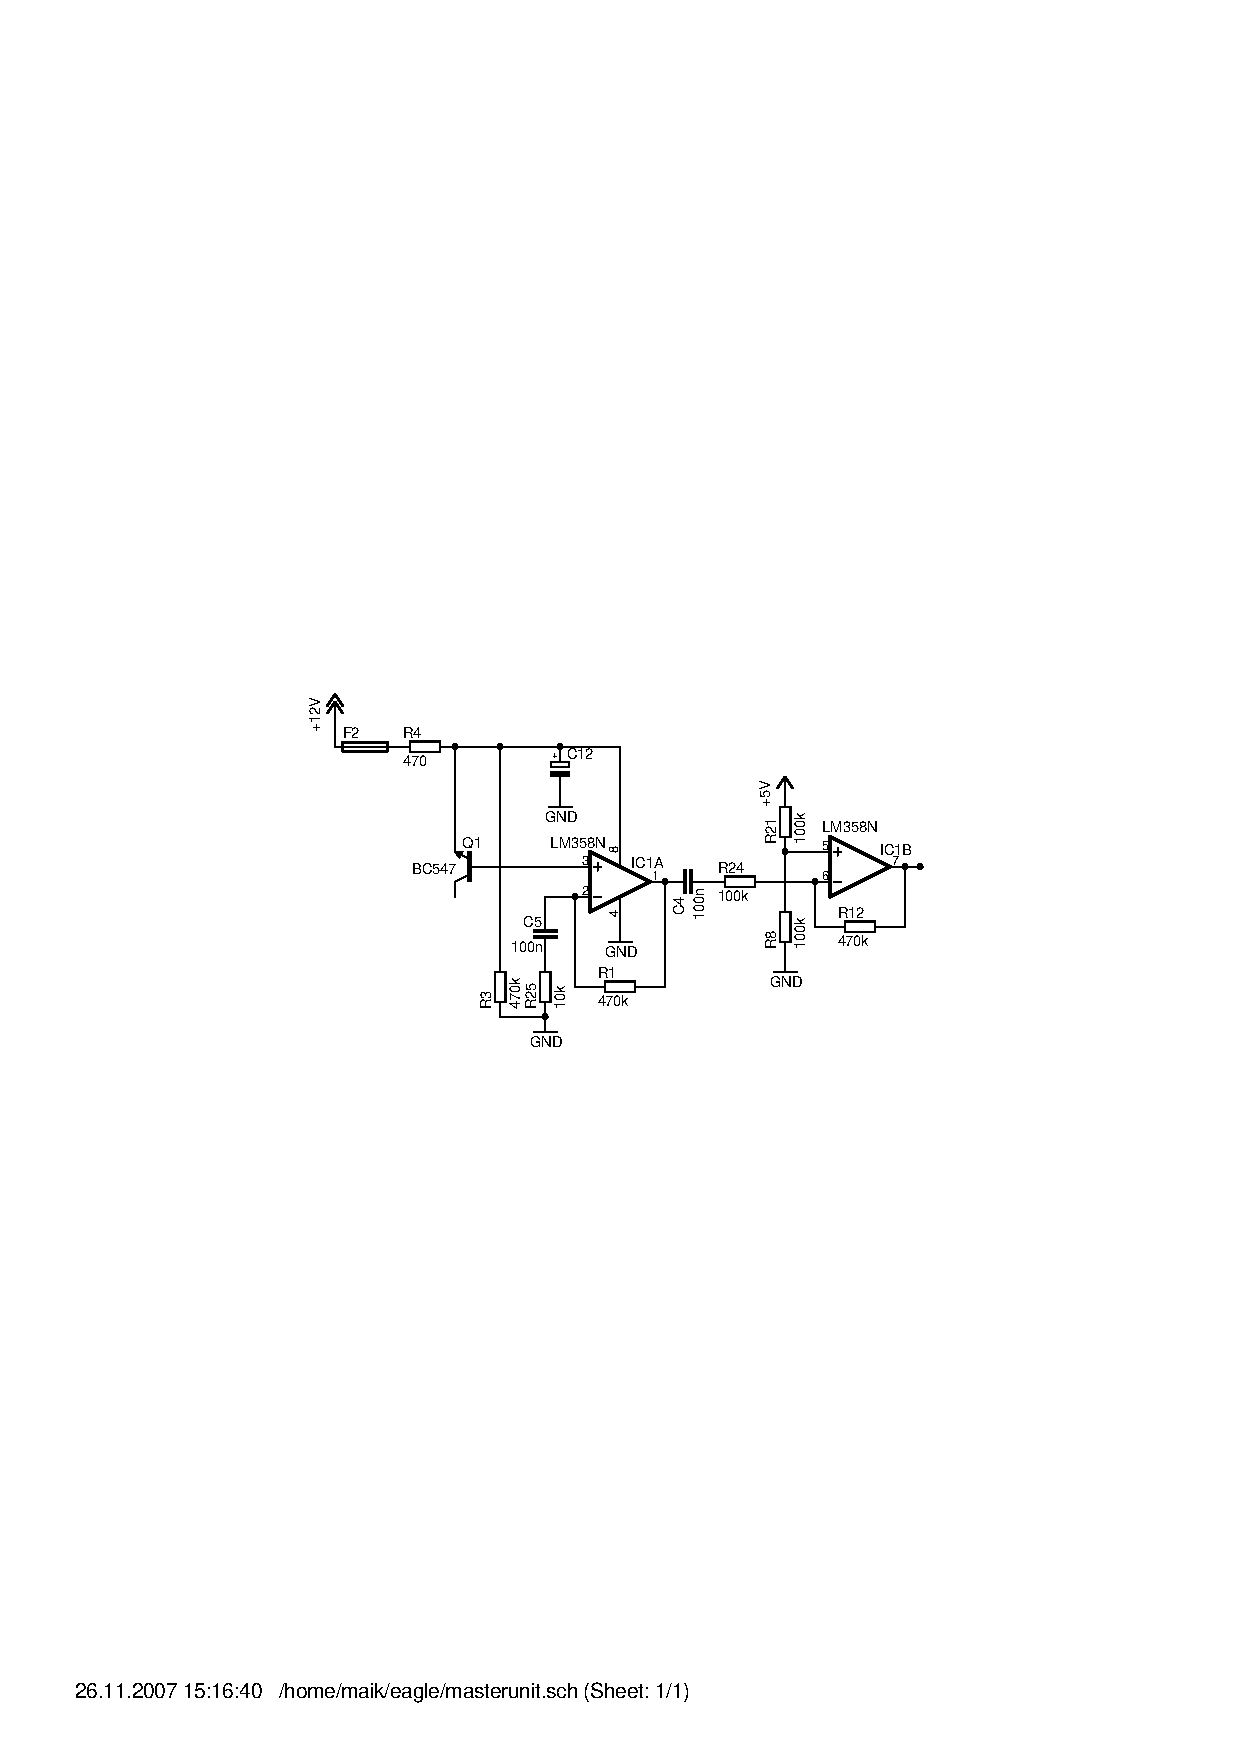
\includegraphics[scale=0.05]{hwrnd_schem}, {schematic of the hardware random generator}]
This curcit utilises the randomnes of the breakthrough voltage of the diode of a transistor to generate random voltages in the range from 0 to 5 volts. While this is quite random it does not need to be cryptographicaly secure because the RNGs output is used only as input for the cryptograpicaly secure PRNG. \\
\end{window}
\vspace{1cm}
%-----

\subsection{pseudornadom number generator (PRNG)}
The PRNG is based on the SHA-256 hash function and is specified in Appendix A.
It has two main functions:
\begin{itemize}
 \item AddEntropy: this function adds data to the entropy pool, the input can be of arbitary bit length
 \item GetRandomBlock: this function fills a 32 byte block of memory with a randomised bitstring
\end{itemize}
An other function (GetRandomByte) uses a buffer and the GetRandomBlock function and returns a random byte.
The PRNG is periodicaly filled with entropy from the hardware RNG using the AddEntropy function.

%-----

\subsection{secure serial port (QPort-tiny)}

%-----

\subsection{external serial eeprom}
The external serial eeprom is used to keep the two databases and can be used for key-exporting for migration. We use standard $I^2C$ EEPROMs with 512KiBit or 1MiBit (24xx512 or 24xx1025) from Microchip. It is possible to extend the storage capabilitys by using multiple EEPROMs. This makes it possible to have up to 4Mbit or 512Kbytes of storage space wich normally allows more than 10,000 users.

The whole contents of the eeprom is encrypted (except the keymigration-area). Shabea-16 is used to encrypt the content. We therefore divide the eeprom space into 32 byte blocks which are encrypted seperatly. Every block is encrypted with an individual key which is the result of concatenation of the ''main-key'' and the blockaddress. So we are protected against most attacks against mass storage encryption (ex. watermarking).

%-----

\subsection{Ticket-Database (TicketDB)}
This database is used to store a HMAC of the users ticket, her/his permissions, and some statistics about the whole system.
The first element in the database is the header followed by the entrys for the users.\\
\begin{tabular}{|l|c|l|}\hline 
name & size & description \\ \hline
ID & 10 bytes & set to the string ''AnonAccess'' \\
majversion & 1 byte & majorversion; set to 1 \\
minversion & 1 byte & minorversion; set to 0 \\
headersize & 1 byte & specifies the size of the header \\
stat & 10 bytes & statistics \\
reserved & 8 bytes & reserved field for future extensions and for alignment; set to 0 \\ \hline
\end{tabular} 

The statistics field has the following structure:\\
\begin{tabular}{|l|c|l|} \hline
name & size & description \\ \hline 
max\_users     & 2 bytes & maximum number of users \\
users              & 2 bytes & actualy active user \\
admins           & 2 bytes & actualy active admins \\
locked\_users   & 2 bytes & number of locked users \\
locked\_admins & 2 bytes & number of locked admins \\ \hline
\end{tabular} 

The following space of the TicketDB is filled with userentrys which have the following structure:\\
\begin{tabular}{|l|c|l|} \hline
name & size & description \\ \hline 
flags         & 1 byte    & the flags associated with the user \\
nickname  & 7 bytess & the nickname if the user decided to be known by name \\
ticketmac  & 32 bytes & HMAC from users ticket \\ \hline
\end{tabular} 

Where the flag field has the following structure: \\
\begin{tabular}{|l|c|l|} \hline
name & size & description \\ \hline 
exists         & 1 bit    &  indicates if this entry is used (1: in use; 0: free)\\
admin  & 1 bit & set if user has admin privileges, cleared othewise \\
locked  & 1 bit & set if user is locked; cleared otherwise \\
noitfy\_lostadmin  & 1 bit & set if user has to be notifyed about lost admin privileges \\
anonymous  & 1 bit & set if the user did not specify username to be stored \\
reserved & 3 bit & reserved, should be set to 0\\ \hline
\end{tabular} 

%-----

\subsection{FlagModifying-Database (FLMDB)}
The FlagModifying-Database keeps entrys which specify how a given useraccount should be modifyed. \\
\begin{tabular}{|l|c|l|} \hline
name & size & description \\ \hline 
active          & 1 byte    & set to 1 if this entry is active; set to 0 othewise \\
permanent  & 1 byte & set to 1 if this entry should not be removed if applied; set to 0 otherwise \\
last             & 1 bytes & if set to 1 this is the last account to check; set to 0 otherwise \\ 
setflags       & 1 byte & specifies which bits have to be set in the userflags\\
clearflags    & 1 byte & specifies which bits have to be cleared in the userflags\\
reserved     & 3 byte & reserved; set to 0\\
timestamp  & 8 bytes & timestamp of the creation of this entry\\
hnick          & 32 bytes & HMAC of the users pseudonym\\
\hline
\end{tabular}

